\chapter{Proposta do Trabalho}
\label{ch:proposta}

Neste capítulo, apresenta-se a proposta de uma abordagem para alocação dinâmica de casos de teste com base no perfil dos testadores envolvidos. Também são apresentadas as atividades já realizadas e as atividades a serem realizadas.Finalizando, apresenta-se o cronograma de execução das atividades a serem realizadas para a conclusão do trabalho. 

\section{Alocação de Casos de Teste Baseado no Perfil de Testadores}

A abordagem proposta para esta pesquisa envolve as seguintes etapas:

\begin{enumerate}
    \item Identificação e levantamento de características pessoais que podem influenciar o processo de teste de software no contexto apresentado; 
    
    \item Extração de informações sobre as características pessoais de cada testador envolvido no processo de teste;
    
    \item Acompanhamento do processo de teste de diversos serviços, com diferentes características, registrando métricas que viabilizam a análise da adequação entre tipos de teste e testadores específicos;
    
    \item Análise dos dados históricos de teste;
    
    \item Definição de \textit{Sistema de Recomendação} que se baseia no conjunto de dados históricos de teste para recomendar casos de teste para testadores;
    
    \item Propor uma estratégia de filtragem para ponderar futuras recomendações, levando em consideração a satisfação do testador durante a realização das atividades de teste.
\end{enumerate}

Cada etapa apresentada consolida uma fase da parte prática deste trabalho, que será executada no TCC2. 

As Seções \ref{sec:caracteristicas_importantes}, \ref{sec:extrair_caracteristicas}, \ref{sec:acompanhar_ciclos} e \ref{sec:analisar_dados} apresentam as principais etapas da abordagem proposta neste trabalho.

\section{Características de Perfil}
\label{sec:caracteristicas_importantes}

Como já apresentado no Capítulo \ref{ch:referencial}, na Seção \ref{sec:perfil_testadores}, a influência da personalidade humana em tarefas individuais é uma das preocupações da Engenharia de Software.  Sendo assim, a influência da personalidade também é uma característica importante deste trabalho, pois configura o mecanismo principal para realização da alocação dos casos de teste dinamicamente.  

A equipe de testadores do ITRAC possui membros com níveis variados de experiência em testes, sendo composta por alunos graduandos em Engenharia de Software,que cursam períodos diferentes do curso, podendo variar entre calouros e veteranos.  Além disso, parte da equipe que realiza os testes nos serviços, utilizando o processo de testes definido pelo ITRAC, é composta por funcionários do ME, já graduados em diferentes cursos, que podem possuir, ou não, uma maior experiência em testes, de um modo geral. 

Esta variação entre os membros da equipe e seus respectivos conhecimentos não é considerada no momento da alocação de casos de teste realizada.  Sendo assim, alunos que estão no início da graduação e sem nenhuma experiência em testes, podem ser alocados a casos de teste que possuem o mesmo nível de dificuldade de casos de teste alocados a testadores experientes. 

Esta falta de critério na alocação de casos de teste pode gerar prejuízos ao processo de Validação do produto de software. Este problema é atacado no trabalho atual, objetivando uma melhor adequação entre os testadores e os casos de teste realizados.

\section{Extração de Informações de Perfil}
\label{sec:extrair_caracteristicas}

Neste trabalho, é necessário extrair as informações sobre o perfil de cada testador da equipe do ITRAC. A extração de informações é feita a partir da utilização de um questionário que foi desenvolvido ao longo deste trabalho com base em \cite{Santos19SDPA}, \cite{geras2004survey} e \cite{groves2000survey}. Baseado nestes trabalhos, foi montado o questionário apresentado no Anexo \ref{anexo:questionario}. 

A criação do questionário foi baseada nas  diretrizes de Kitchenham~\cite{kitchenham2008personal} que apresenta 6 etapas a serem realizadas, como ilustrado na Figura~\ref{fig:Abordagem}.

        \begin{figure}[h]
          \centering
          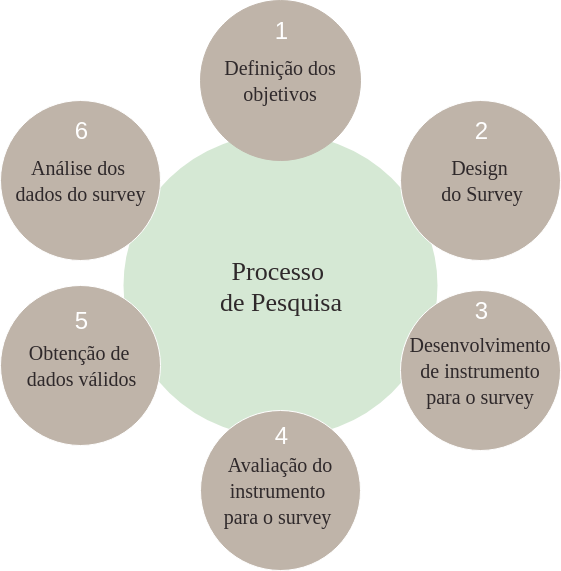
\includegraphics[width=10cm]{figuras/survey.png}
          \caption{Visão geral do processo para elaboração do questionário.  (Fonte: Elaborado pela Autora.)} 
          \label{fig:Abordagem}
        
        \end{figure}
 
 As 6 etapas estão sendo empregadas neste, conforme descrição a seguir:
 
\begin{enumerate} 
\item \textbf{Estabelecer objetivos:} neste trabalho, esta etapa configura o primeiro passo para começar a construir o questionário. Em que cada objetivo é definido;

\item \textbf{Design do \textit{survey}:} o tipo de \textit{design} utilizado neste trabalho é o transversal, onde os participantes serão questionados sobre suas experiências prévias;

\item \textbf{Desenvolvimento de instrumento para o \textit{survey}:} para desenvolver o instrumento, foram empregados os passos: (i) pesquisar a literatura relevante (apresentada no Capítulo \ref{ch:referencial}); (ii) construir um instrumento (Capítulo \ref{ch:metodologia}); (iii) avaliar o instrumento (em produção); e (iv) documentar o instrumento (redação do trabalho como um todo);

\item \textbf{Avaliação do instrumento para o \textit{survey}:} esta avaliação é frequentemente chamada de pré-teste, e possui objetivos distintos: (i) verificar se as questões são compreensíveis; (ii) avaliar a taxa de resposta provável e a eficácia dos procedimentos de acompanhamento; (iii) avaliar a confiabilidade e validade do instrumento; e (iv) garantir que nossa análise de dados as técnicas correspondem às nossas respostas esperadas; 

\item \textbf{Obtenção de dados válidos:} nesta fase é definida uma amostra, que é um subconjunto da população. As respostas deste grupo buscam representar o grupo inteiro. Ao escolher a amostra a ser pesquisada, devemos ter em mente três aspectos do desenho da pesquisa: (i) evitar o viés; (ii) adequação; e (iii) custo-efetividade;

\item \textbf{Análise dos dados do \textit{survey}:} na etapa final, são reunidos todos os dados coletados da pesquisa para extrair informações relevantes para responder às questões definidas nos objetivos da pesquisa e descritas no GQM, destacado na Tabela~\ref{tab:gqm}.
\end{enumerate}
 
Para este trabalho de conclusão de curso (TCC1), foram realizados as 2 primeiras etapas e parte da terceira. O restante das etapas configuram parte do trabalho a ser realizado no TCC2.

\subsection{Design e Questões do Questionário}
\label{sec:desingquestions}

Para projetar o questionário buscou-se na literatura trabalhos similares.

O questionário foi elaborado com base em alguns trabalhos como, por exemplo, o \textit{survey} de~\cite{geras2004survey}, que descreveu os resultados de um \textit{survey} de questionamentos feitos à pessoas envolvidas com o desenvolvimento de software em uma empresa. A partir disso, com o objetivo de caracterizar testes de software e práticas de garantia da qualidade, o questionário foi dividido nas seguintes categorias:

\begin{itemize}
\item  Perfil pessoal e profissional dos respondentes;
\item  Conhecimentos específicos de teste;
\item  Relato livre de experiência;
\end{itemize}

As perguntas referentes à cada categoria podem ser consultadas no Anexo~\ref{anexo:questionario}.

A primeira categoria foi elaborada com o objetivo de coletar informações pessoais e sobre o perfil profissional do respondente, com o interesse em entender o nível de escolaridade, respectivos cursos de graduação, experiências com linguagens de programação e para coletar os usuários de cada testador na ferramenta de gerenciamento de projetos utilizada. No contexto desta pesquisa, foi utilizada a ferramenta \textit{redmine}\footnote{https://www.redmine.org/}. 

A segunda categoria busca entender o grau de familiaridade dos testadores com a atividade de teste. Para isto, o questionário aborda questões sobre técnicas e critérios de teste, por exemplo, para entender como é a experiência dos testadores neste quesito.

A terceira categoria engloba uma questão aberta, que solicita ao testador que relate a sua experiência. Esta questão se faz importante, pois as respostas serão fundamentais para que o testador relate livremente sua experiência, podendo incluir informações que o questionário ainda não contém, mas que são relevantes para a pesquisa. Podendo colaborar, dessa forma, com o aprimoramento do questionário. 

É interessante ressaltar que o questionário ainda está em fase de construção e será aprimorado após uma primeira aplicação com um membro do ME, que também fará parte dos testes dos serviços. Além disso, a aplicação do questionário aos testadores do ITRAC também se faz fundamental colher \textit{feedbacks}.

\section{Acompanhar Ciclos}
\label{sec:acompanhar_ciclos}

O acompanhamento de ciclos deve levar em consideração o registro de determinadas informações. Para tanto, foi necessária a elaboração de um \textit{Goal Question Metric - GQM}, que consiste em um mecanismo utilizado para definir e avaliar um conjunto de objetivos operacionais, utilizando um conjunto de questões e métricas associadas a estes objetivos~\cite{basili1994goal}. O GQM desta pesquisa é apresentado na \ref{tab:gqm}: 

% Please add the following required packages to your document preamble:
% \usepackage[table,xcdraw]{xcolor}
% If you use beamer only pass "xcolor=table" option, i.e. \documentclass[xcolor=table]{beamer}
\begin{table}[htb!]
\label{tab:gqm}
\begin{tabular}{|l|l|}
\hline
\rowcolor[HTML]{C0C0C0} 
\textbf{Goal} & \begin{tabular}[c]{@{}l@{}}Aprimorar o gerenciamento de testes para a atribuição de \\ tarefas de teste com base no perfil do testador\end{tabular} \\ \hline
\rowcolor[HTML]{FFFFFF} 
\textbf{Question 1} & Qual a eficiência da alocação de tarefas de teste para o testador? \\ \hline
\rowcolor[HTML]{FFFFFF} 
\textbf{Métricas} & \begin{tabular}[c]{@{}l@{}}M1: Número de casos de teste gerados pela equipe\\ \\ M2: Número de falhas identificadas pela equipe\\ \\ M3: M2/M1\end{tabular} \\ \hline
\rowcolor[HTML]{EFEFEF} 
\textbf{Question 2} & Qual a eficiência da alocação de casos de teste por parte do testador? \\ \hline
\rowcolor[HTML]{EFEFEF} 
\textbf{Métricas} & \begin{tabular}[c]{@{}l@{}}M1: Número de casos de teste gerados pelo testador\\ 		\\ M4: Número de falhas identificadas por testador\\ 		\\ M5: M4/M3\end{tabular} \\ \hline
\rowcolor[HTML]{FFFFFF} 
\textbf{Question 3} & Qual o impacto do perfil do testador na eficiência dos testes? \\ \hline
\rowcolor[HTML]{FFFFFF} 
\textbf{Métrica} & M5: Variação entre a eficiência de cada testador \\ \hline
\rowcolor[HTML]{EFEFEF} 
\textbf{Question 4} & Qual o grau de satisfação do testador durante o ciclo de teste? \\ \hline
\rowcolor[HTML]{EFEFEF} 
\textbf{Métrica} & M6: Grau de satisfação (0 a 5) \\ \hline
\rowcolor[HTML]{FFFFFF} 
\textbf{Question 5} & Qual a eficiência dos testes em relação a cada tour? \\ \hline
\rowcolor[HTML]{FFFFFF} 
\textbf{Métrica} & M6 (tour 1) = M1(tour 1)/M4(tour1) \\ \hline
\end{tabular}
\end{table}

Dadas as etapas destacadas, a Seção \ref{sec:abordagem} apresenta a abordagem proposta neste trabalho.

\section{Abordagem}
\label{sec:abordagem}

A abordagem proposta nesta pesquisa envolve um processo contínuo de aprendizado e evolução, que depende de diversos ciclos de teste em diferentes tipos de serviço. O contexto no qual o laboratório ITRAC se encontra viabiliza a aplicação de tal abordagem, dada as características de um processo de transformação digital em grande escala. 
        
O processo de transformação digital do governo brasileiro envolve um grande número de serviços de baixa complexidade, o que possibilita um grande número de ciclos de teste em um curto período de tempo. Tal característica favorece o aprendizado e a evolução relacionada as atividades de teste neste contexto. 
		
A partir das métricas destacadas na Tabela \ref{tab:gqm}, é possível que análises sejam realizadas buscando uma melhora contínua da atividade de alocação de casos de teste.

Neste sentido, a Figura \ref{fig:Abordagem} apresenta o processo contínuo de aprendizado, juntamente com a abordagem proposta para este trabalho. Foi utilizado o \textit{lemniscate} – figura do número 8 virada para representar o processo.

        \begin{figure}[h]
          \centering
          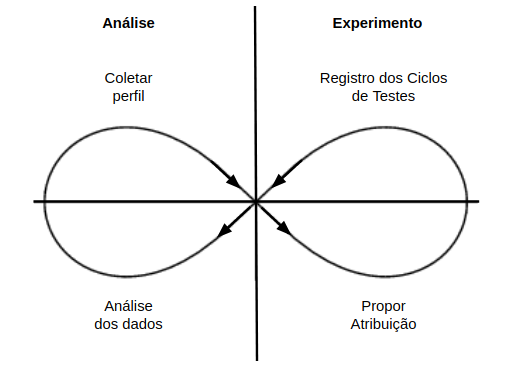
\includegraphics[width=13cm]{figuras/abordagem.png}
          \caption{Abordagem para o Sistema de Recomendação  (Fonte: Elaborado pela Autora.)} 
          \label{fig:Abordagem}
        
        \end{figure}		
		
	
A parte esquerda da figura relaciona-se com a Análise e está vinculada à coleta do perfil do testador e à análise dos dados coletados depois de cada ciclo de teste. Enquanto a parte direita relaciona o que se pretende usar como experimento, que configura o registro dos ciclos de teste e a proposta de alocação. A seguir, serão descritas cada fase da abordagem:

\subsection{Coletar Perfil}

Como apresentado na Seção~\ref{sec:caracteristicas_importantes}, as características de perfil de cada testador serão levadas em consideração para a constituição deste trabalho. Para dar início às partes práticas será necessário coletar o perfil dos testadores envolvidos. O perfil de cada testador será traçado a partir da extração de informações do perfil obtidas a partir do questionário já apresentado na Seção \ref{sec:extrair_caracteristicas}.

O questionário será refinado até estabelecer as questões necessárias para consolidar um perfil que contenha as informações necessárias do usuário sobre cada categoria apresentada na Subseção \ref{sec:desingquestions}. Após a consolidação deste perfil, uma página de perfil para cada testador será criada na ferramenta \itractool para que os testadores tenham um cadastro com todas as informações coletadas. 

\subsubsection{Cadastrar perfil na ferramenta \itractool}

É importante que os testadores tenham seus perfis individuais cadastrados na ferramenta, pois estes perfis irão fornecer a informação sobre o domínio dos testadores sobre testes. Estas informações serão registradas no banco de dados e serão atualizadas de acordo com a realização dos cilos de teste. 

Com as informações cadastradas será possível traçar, baseado em dados históricos, qual o \textit{tour} e o caso de teste mais adequado para cada perfil de testador, levando em consideração a experiência do testador com o teste exploratório dos serviços. A partir disso, será possível predizer quais atividades de teste ele está executando com mais eficiência para poder realizar uma melhor alocação de atividades de teste. O perfil ideal para o testador seria aquele que conseguisse captar além das características técnicas, a experiência naquele domínio de aplicação para, em seguida, propor uma alocação. 

\subsection{Propor Alocação}
 
 Esta fase consiste na proposta de alocação baseada em perfil, ou seja, uma página de um serviço com determinados campos e características específicas pode ter um caso de teste e um testador ideal. O sistema de recomendação sugere quais casos de teste são adequados para determinado testador utilizar baseado em seu histórico de testes já realizados. A partir disso, a página e campos em questão são testados.
 
 Os sistemas de recomendação, como já explicitado no Capítulo \ref{ch:referencial}, na Seção \ref{sec:sistemas}, realizam filtragens de informações que recomendam itens aos usuários. No caso deste trabalho o item é uma alocação de caso de teste para um testador. 
 
 A alocação de casos de teste e testadores deve ser realizada de maneira dinâmica, com um processo de aprendizado durante cada ciclo de teste. Ou seja, a alocação dos casos de teste e dos testadores deve levar em consideração, além das características já citadas, o aprendizado obtido ao longo dos ciclos de teste anteriores. O aprendizado citado busca maximizar a eficiência da aplicação dos casos de teste. Neste contexto, a palavra ``eficiência'' faz referência a taxa de identificação de falhas durante a aplicação dos casos de teste. Desse modo, a ``eficiência'' é dada pela Equação \ref{eq:eficiencia}.
 
 \begin{equation}
 \label{eq:eficiencia}
    eficiencia = \frac{numero \ de \ falhas\ identificadas}{numero\ de\ casos\ de\ teste}    
 \end{equation}
 
 
Neste trabalho, assim como proposto em~\cite{miranda2012recommender}, a alocação é representada como um par caso de teste e testador, representado por \{CTn;Tn\} (Caso de Teste \emph{n} e Testador \emph{n}). O usuário é representado por um típico gerente de teste e as recomendações são feitas comparando um caso de teste específico com o perfil de um testador e avaliando sua similaridade.
 
 Após a alocação e a realização dos casos de teste alocados, surge a etapa de registro dos casos de teste, detalhada a seguir.
 
\section{Registro dos Ciclos de Teste}

Os casos de teste realizados pelos testadores do ITRAC já são registrados na ferramenta \textit{Redmine}. Estes casos de teste já possuem um padrão a ser seguido para terem suas informações guardadas. Com isso, a obtenção dos casos de teste realizados pode ser feita a partir da API (\textit{Application Programming Interface}) do \textit{Redmine}. 

A Figura \ref{fig:registro} apresenta a estrutura organizacional atual dos registros realizados no \textit{Redmine}. 


        \begin{figure}[h]
          \centering
          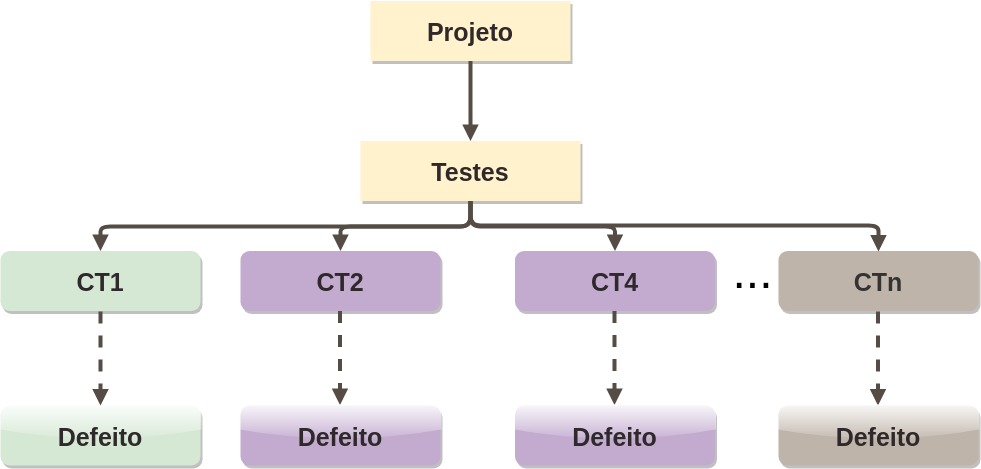
\includegraphics[width=15cm]{figuras/registro.png}
          \caption{Estrutura Organizacional dos Registros no \textit{Redmine}. (Fonte: Elaborado pela Autora.)} 
          \label{fig:registro}
        
        \end{figure}		

Na Figura \ref{fig:registro}, \textbf{Projeto} representa um serviço digitizado, que foi registrado no \textit{Redmine}. \textbf{Testes} representam o conjunto de casos de teste associados ao projeto. O conjunto de testes é definido à partir do conceito de \textit{tasks} do \textit{Redmine}. A definição desta entidade que agrupa os casos de teste se deu para facilitar a obtenção de informações de maneira agrupada, viabilizando, por exemplo, a extração do status de conclusão do conjunto de casos de teste como um todo.

Os \textbf{CTs} representam os casos de teste registrados no \textit{Redmine}. Estes são definidos a partir do conceito de \textit{subtasks} associados à \textit{task} \textbf{Testes} e possuem os atributos apresentados na Tabela \ref{tab:atributo}.

% Please add the following required packages to your document preamble:
% \usepackage[table,xcdraw]{xcolor}
% If you use beamer only pass "xcolor=table" option, i.e. \documentclass[xcolor=table]{beamer}
\begin{table}[H]
\centering
\caption{Atributos dos Casos de Teste Registrados no \textit{Redmine}.}
\label{tab:atributo}
\begin{tabular}{|l|l|}
\hline
\textbf{Atributo} & \textbf{Descrição} \\ \hline
Título & Registra o título do caso de teste \\ \hline
\rowcolor[HTML]{EFEFEF} 
Data de criação & Registra a data de criação do teste \\ \hline
Data de execução & Registra a data da execução do teste \\ \hline
\rowcolor[HTML]{EFEFEF} 
Tempo para execução & \begin{tabular}[c]{@{}l@{}}Registra o tempo gasto para realizar \\ o caso de teste\end{tabular} \\ \hline
Tour utilizada & Registra a tour utilizada para o caso de teste \\ \hline
\rowcolor[HTML]{EFEFEF} 
\begin{tabular}[c]{@{}l@{}}Quantidade de \\ campos envolvidos\end{tabular} & \begin{tabular}[c]{@{}l@{}}Registra quantos campos estão envolvidos\\  no caso de teste\end{tabular} \\ \hline
Testador responsável & \begin{tabular}[c]{@{}l@{}}Registra o testador responsável pela execução\\ do caso de teste\end{tabular} \\ \hline
\rowcolor[HTML]{EFEFEF} 
Resultado & \begin{tabular}[c]{@{}l@{}}Registra o resultado final da execução do\\ caso de teste (sucesso, ou falha)\end{tabular} \\ \hline
Entrada & Registra as entradas aplicadas ao caso de teste \\ \hline
\rowcolor[HTML]{EFEFEF} 
Saída esperada & Registra a saída esperada para o caso de teste \\ \hline
Saída obtida & \begin{tabular}[c]{@{}l@{}}Registra a saída obtida durante a aplicação\\ do caso de teste\end{tabular} \\ \hline
\rowcolor[HTML]{EFEFEF} 
Descrição & Registra a descrição do caso de teste \\ \hline
\end{tabular}
\end{table}

Os \textbf{Defeitos} são definidos como \textit{subtasks} das \textit{subtasks} \textbf{CTs} e possuem os atributos apresentados na Tabela \ref{tab:defeito}. Vale ressaltar que os \textbf{CTs} podem possuir, ou não, um \textbf{Defeito} associado. Essa possibilidade de ter ou não um Defeito associado é representado, na Figura \ref{fig:registro}, a partir da utilização de setas trastejadas.

% Please add the following required packages to your document preamble:
% \usepackage[table,xcdraw]{xcolor}
% If you use beamer only pass "xcolor=table" option, i.e. \documentclass[xcolor=table]{beamer}
\begin{table}[H]
\centering
\caption{Atributos dos Defeitos Registrados no \textit{Redmine}.}
\label{tab:defeito}
\begin{tabular}{|l|l|}
\hline
\textbf{Atributo} & \textbf{Descrição} \\ \hline
\rowcolor[HTML]{FFFFFF} 
Título & Registra o título do defeito \\ \hline
\rowcolor[HTML]{EFEFEF} 
Prioridade & Registra o nível de prioridade para a resolução do defeito \\ \hline
\rowcolor[HTML]{FFFFFF} 
Categoria & Registra a categoria a qual o defeito pertence \\ \hline
\rowcolor[HTML]{EFEFEF} 
Tipo de falha & Registra o tipo de falha encontrada \\ \hline
\rowcolor[HTML]{FFFFFF} 
\begin{tabular}[c]{@{}l@{}}Passos para \\ reproduzir o bug\end{tabular} & Registra os passos que levaram à ocorrência da falha \\ \hline
\rowcolor[HTML]{EFEFEF} 
Provas visuais & \begin{tabular}[c]{@{}l@{}}Registra os defeitos encontrados, geralmente, em forma \\ de \textit{prints}, como prova visual\end{tabular} \\ \hline
\rowcolor[HTML]{FFFFFF} 
Ambiente & \begin{tabular}[c]{@{}l@{}}Registra em qual sistema operacional, resolução da tela,\\ browser e nível de zoom o a falha ocorreu\end{tabular} \\ \hline
\end{tabular}
\end{table}

Em relação ao atributo \textbf{Tipo de Falha}, vale destacar que os tipos definidos até o momento são: 1) Regra de Negócio, 2) Interface e 3) Validação de Campos. 

\section{Análise dos Dados}
\label{sec:analisar_dados}

Com base na análise do GQM, a intenção é verificar a existência de uma correlação entre a eficiência no processo de teste e as diferentes variáveis que compõem o perfil dos testadores. Este perfil será identificado com base em diferentes questões respondidas pelos testadores num questionário digital, como o apresentado no Anexo~\ref{anexo:questionario}. 

Ao obter as questões respondidas do questionário, o passo seguinte é coletar os dados sobre a eficiência de cada testador na realização das atividades de teste. Para que se colete estes dados, é possível a realização de testes de correlação para identificar se há alguma relação entre as variáveis do perfil e a eficiência nos testes de determinado testador ou da equipe de testes como um todo.

Baseado nos dados, pode-se retomar à pergunta de pesquisa e entender: \textbf{Qual o impacto das variáveis do perfil do testador na eficiência dos testes?} A partir desta fase, é possível utilizar o questionário para fazer um teste de correlação entre as variáveis levantadas.


\section{Integração \itractool}

Este trabalho propõe a inclusão de um novo módulo na ferramenta \itractool, apresentada na Seção \ref{sec:dtest}. A integração deste módulo segue o apresentado na Figura \ref{img:architecture2}.

\begin{figure}[H]
  \centering
  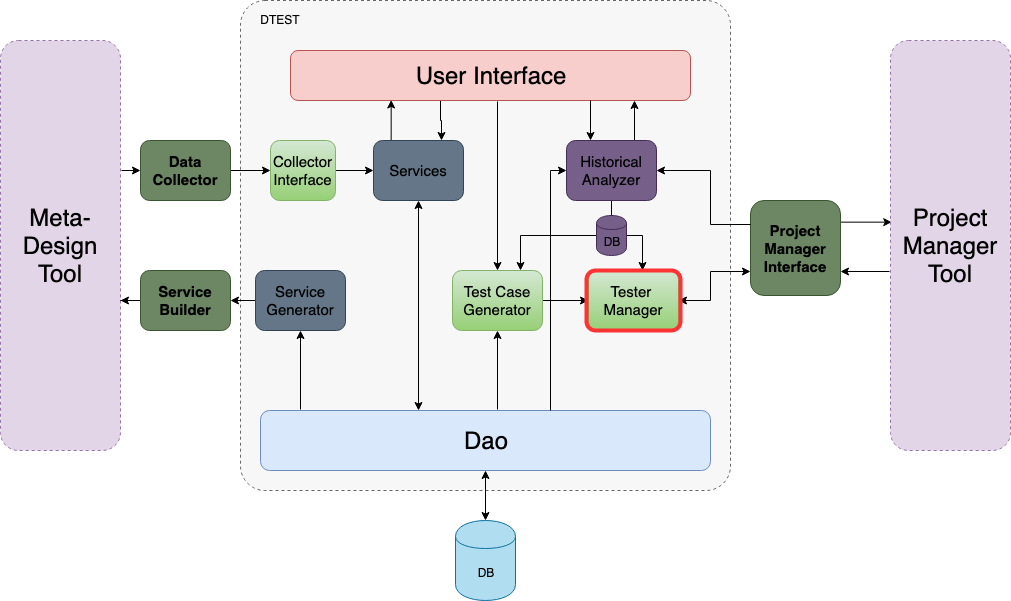
\includegraphics[width=14cm]{figuras/arquitetura.png}
  \caption{Arquitetura \itractool após a inclusão do módulo \textit{Tester Manager}.)} 
  \label{img:architecture2}
\end{figure}

O módulo proposto, chamado de \textbf{Tester Manager}, utiliza como \textit{input} informações advindas dos módulos \textbf{Test Case Generator} (TCG) e \textbf{Historical Analyzer} (HA), além de informações diretamente obtidas a partir da ferramenta de gerenciamento de projetos utilizada.

O módulo TCG exporta o caso de teste que deverá ser alocado entre os testadores disponíveis. O módulo \textbf{Tester Manager}, com base nas informações de perfil de cada testador, deverá associar o testador que mais se adéqua ao caso de teste em questão. Para isso, informações histórias da execução de casos de teste são utilizadas como base de conhecimento. Um processo de aprendizado utilizando esta base de conhecimento viabiliza a implementação de um \textit{Sistema de Recomendação} que seja capaz de recomendar o testador mais adequado para determinado caso de teste.